\documentclass[landscape,final,columns=3]{baposter}
\usepackage{geometry}
\geometry{left=0.8in,right=0.8in,top=0.8in,bottom=0.8in}
\usepackage{times}
\usepackage{calc}
\usepackage{graphicx}
\usepackage{amsmath}
\usepackage{amssymb}
\usepackage{amsthm}
\usepackage{relsize}
\usepackage{multirow}
\usepackage{bm}
\usepackage{color}
\usepackage{framed}

\usepackage{amsmath}
\usepackage{amsfonts}
\usepackage{amsthm}
\usepackage{enumitem}
\usepackage{dsfont}
\usepackage{amssymb}
\usepackage{pifont}
\usepackage{mathtools}

\newtheorem{thm}{Theorem}[section]
\newtheorem{lem}[thm]{Lemma}
\newtheorem{prop}[thm]{Proposition}
\newtheorem{conj}[thm]{Conjecture}
\newtheorem{cor}[thm]{Corollary}

\newtheorem*{prop*}{Proposition}

\theoremstyle{definition}
\newtheorem{claim}[thm]{Claim}
\newtheorem{defn}[thm]{Definition}
\newtheorem{quest}[thm]{Question}
\newtheorem{remark}[thm]{Remark}
\newtheorem{fact}[thm]{Fact}
\newtheorem{note}[thm]{Note}

\newtheorem*{claim*}{Claim}
\newtheorem*{quest*}{Question}
\newtheorem*{remark*}{Remark}
\newtheorem*{fact*}{Fact}

\newcommand{\N}{\ensuremath{\mathbb{N}}}
\newcommand{\Z}{\ensuremath{\mathbb{Z}}}
\newcommand{\Q}{\ensuremath{\mathbb{Q}}}
\newcommand{\R}{\ensuremath{\mathbb{R}}}
\newcommand{\C}{\ensuremath{\mathbb{C}}}
\newcommand{\F}{\ensuremath{\mathbb{F}}}
\newcommand{\AP}{\ensuremath{\mathcal{A}_{2^{n}}}}
\newcommand{\BP}{\ensuremath{\mathcal{B}_{2^{n}}}}
\newcommand{\CP}{\ensuremath{\mathcal{C}_{2^{n}}}}
\newcommand{\DP}{\ensuremath{\mathcal{D}_{2^{n}}}}
\newcommand{\EP}{\ensuremath{\mathcal{E}_{2^{n}}}}
\newcommand{\FP}{\ensuremath{\mathcal{F}_{2^{n}}}}

\newcommand{\E}{\ensuremath{\mathbb{E}}}
\newcommand{\1}{\ensuremath{\mathds{1}}}

\newcommand{\pair}[2]{\ensuremath{\langle #1, #2 \rangle}}

\DeclareMathOperator{\Gal}{Gal}
\DeclareMathOperator{\Jac}{Jac}
\DeclareMathOperator{\Var}{Var}
\DeclareMathOperator{\Cov}{Cov}
\DeclareMathOperator{\Div}{Div}
\DeclareMathOperator{\Prin}{Prin}        
\DeclareMathOperator{\im}{im}
\DeclareMathOperator{\val}{val}

\usepackage{graphicx}
\usepackage{multicol}

\usepackage{pgfbaselayers}
\pgfdeclarelayer{background}
\pgfdeclarelayer{foreground}
\pgfsetlayers{background,main,foreground}

\usepackage{helvet}
\usepackage{palatino}
\pagestyle{empty}
\newcommand{\captionfont}{\footnotesize}

\usepackage{xcolor}
\pagecolor[RGB]{255,254, 230}

\selectcolormodel{cmyk}

\graphicspath{{images/}}
\setlength{\columnsep}{0.7em}
\setlength{\columnseprule}{0mm}
\newcommand{\compresslist}{%
\setlength{\itemsep}{1pt}%
\setlength{\parskip}{0pt}%
\setlength{\parsep}{0pt}%
}

\begin{document}

\typeout{Poster Starts}
%by changing the values inside the curly brackets you can get new colors
\definecolor{mit}{cmyk}{0,.667,.667,.4}
\definecolor{wil}{cmyk}{0.5,1,0,.6}
\definecolor{silver}{cmyk}{0,0,0,0.3}
\definecolor{yellow}{cmyk}{0,0,0.9,0.0}
\definecolor{reddishyellow}{cmyk}{0,0.22,1.0,0.0}
\definecolor{black}{cmyk}{0,0,0.0,1.0}
\definecolor{darkYellow}{cmyk}{0,0,1.0,0.5}
\definecolor{darkSilver}{cmyk}{0,0,0,0.1}
\definecolor{lightyellow}{cmyk}{0,0,0.3,0.0}
\definecolor{lighteryellow}{cmyk}{0,0,0.1,0.0}
\definecolor{lightestyellow}{cmyk}{0,0,0.05,0.0}
\begin{poster}{
  grid=no,
  columns=3,
   colspacing=1em,
  bgColorOne=lighteryellow, %background inside the boxes
  bgColorTwo=lightestyellow, %background color
  borderColor=reddishyellow,
  headerColorOne=yellow,
  headerColorTwo=reddishyellow,
  headerFontColor=black,
  boxColorOne=lightyellow,
  boxColorTwo=lighteryellow,
  % Format of textbox
  textborder=roundedleft,
  % Format of text header
  eyecatcher=no,
  headerborder=open,
  headerheight=0.08\textheight,
  headershape=roundedright,
  headershade=plain,
  headerfont=\Large\textsf, %Sans Serif
  boxshade=plain,
  background=plain,
  linewidth=2pt
  }
  {
  }
{\bf{\textcolor{mit}{The Jacobian group of a finite graph and the monodromy pairing}} %title
  % Authors
{\rm \\ \large  Louis Gaudet, Nicholas Wawrykow, and Theodore Weisman \ \ \
 \textbf{Mentors:} Daniel Corey, David Jensen, and Dhruv Ranganathan \\
 SUMRY 2014,\ Yale University
  }}

  % University logo: change the CMU.jpeg to whatever picture you want and then uncomment this section
%  {
%   \makebox[8em][r]{
%      \begin{minipage}{16em}
%        \hfill
%        \includegraphics[height=6.5em]{mitsealY.eps}
%            \end{minipage}
%            \hspace{-1.35in}
%        \begin{minipage}{16em}
%        \hfill
%        \includegraphics[height=5.8em]{wilsealY.eps}
%            \end{minipage}
%         \hspace{-1.35in}
%        \begin{minipage}{16em}
%        \hfill
%        \includegraphics[height=5.8em]{cookie.eps}
%            \end{minipage}
%    }
%  }

  \tikzstyle{light shaded}=[top color=baposterBGtwo!30!white,bottom color=baposterBGone!30!white,shading=axis,shading angle=30]
     \newlength{\leftimgwidth}
     \setlength{\leftimgwidth}{0.78em+8.0em}

%%%%%%%%%%%%%%%%%%%%%%%%%%%%%%%%%%%%%%%%%%%%%%%%%%%%%%%%%%%%%%%%%%%%%%%%%%%%%%
%%% Now define the boxes that make up the poster
%%%---------------------------------------------------------------------------
%%% Each box has a name and can be placed absolutely or relatively.
%%% The only inconvenience is that you can only specify a relative position
%%% towards an already declared box. So if you have a box attached to the
%%% bottom, one to the top and a third one which should be in between, you
%%% have to specify the top and bottom boxes before you specify the middle
%%% box.
%%%%%%%%%%%%%%%%%%%%%%%%%%%%%%%%%%%%%%%%%%%%%%%%%%%%%%%%%%%%%%%%%%%%%%%%%%%%%%
    %
    % A colored circle useful as a bullet with an adjustably strong filling
    \newcommand{\colouredcircle}[1]{%
      \tikz{\useasboundingbox (-0.2em,-0.32em) rectangle(0.2em,0.32em); \draw[draw=black,fill=baposterBGone!80!black!#1!white,line width=0.03em] (0,0) circle(0.18em);}}


 
 %%%%%%%%%%%%%%%%%%%%%%%%%%%%%%%%%%%%%%%%%%%%%%%%%%%%%%%%%%%%%%%%%%%%%%%%%%%%%%
  \headerbox{{\bf{Acknowledgements}}}{name=ack,column=0,span=2,above=bottom}{
%%%%%%%%%%%%%%%%%%%%%%%%%%%%%%%%%%%%%%%%%%%%%%%%%%%%%%%%%%%%%%%%%%%%%%%%%%%%%%
  \smaller
  This research was conducted as part of the 2014 SUMRY program at Yale University. We would like to thank Sam Payne for our funding, and our mentors as well as Sam Payne, Nathan Kaplan, and Anup Rao for many helpful conversations and for their guidance.
}%

%%%%%%%%%%%%%%%%%%%%%%%%%%%%%%%%%%%%%%%%%%%%%%%%%%%%%%%%%%%%%%%%%%%%%%%%%%%%%%
  \headerbox{{{\bf{The Jacobian group of a graph}}}}{name=defs,column=0,row=0,above=ack}{
  
{\textcolor{purple}{\large{\bf{Divisors on a graph}}}} \vspace{0.05in}\\
Let $G$ be a finite, connected multigraph with no loop edges. Let $V(G),E(G)$ be the vertex and edge sets of $G$.

\begin{itemize}
\item a \textbf{divisor} is an element of $\Div(G)=\bigoplus_{v\in V(G)}\Z(v)$, the free abelian group generated by $V(G)$
\end{itemize}
We think of divisors as ``configurations of chips'' on the vertices of $G$, with group structure given by pointwise addition:

\begin{center}
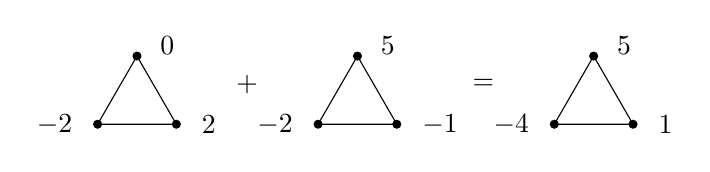
\begin{tikzpicture}

%first divisor
\draw (60:1) -- (0,0) -- (0:1) -- (60:1) ;

\draw [fill] (0,0) circle [radius=0.05cm] ;
\draw [fill] (60:1) circle [radius=0.05cm] ;
\draw [fill] (0:1) circle [radius=0.05cm] ;

%first divisor labels
\node [right] at (60:1.15) {$\;0$} ;
\node [left] at (-.1,0) {$-2\;$} ;
\node [right] at (0:1.2) {$2$} ;

%second divisor
\draw [shift={(2.8cm,0cm)}] (60:1) -- (0,0) -- (0:1) -- (60:1) ;

\draw [fill,shift={(2.8cm,0cm)}] (0,0) circle [radius=0.05cm] ;
\draw [fill,shift={(2.8cm,0cm)}] (60:1) circle [radius=0.05cm] ;
\draw [fill,shift={(2.8cm,0cm)}] (0:1) circle [radius=0.05cm] ;

%second divisor labels
\node [right,shift={(2.8cm,0cm)}] at (60:1.15) {$\;5$} ;
\node [left,shift={(2.8cm,0cm)}] at (-.1,0) {$-2\;$} ;
\node [right,shift={(2.8cm,0cm)}] at (0:1.2) {$-1$} ;

%resulting divisor
\draw [shift={(5.8cm,0cm)}] (60:1) -- (0,0) -- (0:1) -- (60:1) ;

\draw [fill,shift={(5.8cm,0cm)}] (0,0) circle [radius=0.05cm] ;
\draw [fill,shift={(5.8cm,0cm)}] (60:1) circle [radius=0.05cm] ;
\draw [fill,shift={(5.8cm,0cm)}] (0:1) circle [radius=0.05cm] ;

%resulting divisor labels
\node [right,shift={(5.8cm,0cm)}] at (60:1.15) {$\;5$} ;
\node [left,shift={(5.8cm,0cm)}] at (-.1,0) {$-4\;$} ;
\node [right,shift={(5.8cm,0cm)}] at (0:1.2) {$1$} ;

%plus and equals signs
\node [shift={(1.9cm,-.5cm)}] at (0,1) {$+$} ;
\node [shift={(4.9cm,-.5cm)}] at (0,1) {$=$} ;

\end{tikzpicture}
\end{center}

{\textcolor{purple}{\large{\bf{Chip-firing}}}} \vspace{0.05in}\\
You can ``fire'' a vertex on a divisor to get a new divisor:

\begin{center}
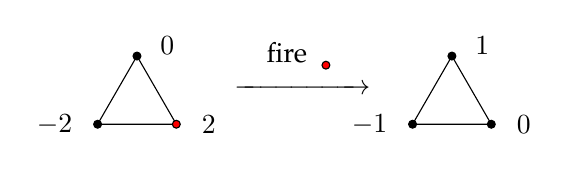
\begin{tikzpicture}

%first divisor
\draw (60:1) -- (0,0) -- (0:1) -- (60:1) ;

\draw [fill] (0,0) circle [radius=0.05cm] ;
\draw [fill] (60:1) circle [radius=0.05cm] ;
\draw [fill=red] (0:1) circle [radius=0.05cm] ;

%first divisor labels
\node [right] at (60:1.15) {$\;0$} ;
\node [left] at (-.1,0) {$-2\;$} ;
\node [right] at (0:1.2) {$2$} ;

%fire arrow
\node [shift={(2.6cm,-.5cm)}] at (0,1) {$\xrightarrow{\hspace{1.5cm}}$} ;
\node [above,shift={(2.6cm,-.5cm)}] at (0,1.15) {fire\;\;\;\;} ;
\draw [fill=red,shift={(2.9cm,1cm)}] (0,-.25) circle [radius=0.05cm] ;

%second divisor
\draw [shift={(4cm,0cm)}] (60:1) -- (0,0) -- (0:1) -- (60:1) ;

\draw [fill,shift={(4cm,0cm)}] (0,0) circle [radius=0.05cm] ;
\draw [fill,shift={(4cm,0cm)}] (60:1) circle [radius=0.05cm] ;
\draw [fill,shift={(4cm,0cm)}] (0:1) circle [radius=0.05cm] ;

%second divisor labels
\node [right,shift={(4cm,0cm)}] at (60:1.15) {$\;1$} ;
\node [left,shift={(4cm,0cm)}] at (-.1,0) {$-1\;$} ;
\node [right,shift={(4cm,0cm)}] at (0:1.2) {$0$} ;

\end{tikzpicture}
\end{center}

If you can get between two divisors $D$ and $D'$ via a sequence of chip-firing moves, then $D,D'$ are equivalent, $D\sim D'$.

\vspace{0.1in}

{\textcolor{purple}{\large{\bf{The Jacobian group}}}}
\begin{itemize}
\item $\deg(D)=$ the total number of chips in $D$
\item $\Div^0(G)=\{D\in\Div(G):\deg(D)=0\}$
\end{itemize}
Now we define the \textbf{Jacobian} group of the graph $G$:
\[
\Jac(G) = \Div^0(G)/\sim.
\]
For a finite graph $G$, $\Jac(G)$ is a finite abelian group.

\begin{fact*}
$|\Jac(G)|=$ the number of spanning trees of $G$.
\end{fact*}
This fact is a consequence of the Matrix Tree Theorem.

\vspace{0.1in}

 }

%%%%%%%%%%%%%%%%%%%%%%%%%%%%%%%%%%%%%%%%%%%%%%%%%%%%%%%%%%%%%%%%%%%%%%%%%%%%%%
 \headerbox{{\bf{Pairings on finite abelian groups}}}{name=pair,span=1,column=1,row=0}{
%%%%%%%%%%%%%%%%%%%%%%%%%%%%%%%%%%%%%%%%%%%%%%%%%%%%%%%%%%%%%%%%%%%%%%%%%%%%%%

Given a finite abelian group $\Gamma$, a \textbf{pairing} on $\Gamma$ is an inner-product like structure $\pair{\cdot}{\cdot}:\Gamma\times\Gamma \to \Q/\Z$ that is \emph{symmetric}, \emph{bilinear}, and \emph{non-degenerate}.

\vspace{0.165in}

{\textcolor{purple}{\large{\bf{Orthogonal sum}}}} \vspace{0.05in}\\
Given two groups $\Gamma_1,\Gamma_2$ with pairings $\pair{\cdot}{\cdot}_1,\pair{\cdot}{\cdot}_2$, the \textbf{orthogonal sum} is a natural pairing defined on $\Gamma_1\times\Gamma_2$ by
\[
\pair{(a_1,a_2)}{(b_1,b_2)}=\pair{a_1}{b_1}_1+\pair{a_2}{b_2}_2.
\]

\vspace{0.065in}

}

%%%%%%%%%%%%%%%%%%%%%%%%%%%%%%%%%%%%%%%%%%%%%%%%%%%%%%%%%%%%%%%%%%%%%%%%%%%%%%
 \headerbox{{\bf{Pairings on $\Z/p^r\Z$}}}{name=prpair,span=1,column=2,row=0}{
%%%%%%%%%%%%%%%%%%%%%%%%%%%%%%%%%%%%%%%%%%%%%%%%%%%%%%%%%%%%%%%%%%%%%%%%%%%%%%

If $p$ is an odd prime, then, up to isomorphism, there are precisely two pairings on $\Z/p^r\Z$. Written additively, they are given by
\vspace{-0.15in}
\[
\pair{x}{y}=xy/p^r \quad \text{and} \quad \pair{x}{y}=axy/p^r,
\vspace{-0.05in}
\]
where $a$ is some quadratic nonresidue modulo $p^r$. We call these the \textbf{residue} and \textbf{nonresidue} pairings, respectively.

\vspace{0.1in}

{\textcolor{purple}{\large{\bf{Classification theorem}}}} \vspace{0.05in}\\
Given any pairing on any finite abelian group of \emph{odd} order, we can write it as the orthogonal sum of pairings on $\Z/p^r\Z$ terms.

}

%%%%%%%%%%%%%%%%%%%%%%%%%%%%%%%%%%%%%%%%%%%%%%%%%%%%%%%%%%%%%%%%%%%%%%%%%%%%%%
  \headerbox{{\bf{The monodromy pairing on the Jacobian}}}{name=2rpair,column=1, span=2, above=ack,below=pair,below=prpair}{
%%%%%%%%%%%%%%%%%%%%%%%%%%%%%%%%%%%%%%%%%%%%%%%%%%%%%%%%%%%%%%%%%%%%%%%%%%%%%%

\begin{multicols}{2}

Given a graph $G$, $\Jac(G)$ is endowed with a canonical pairing called the \textbf{monodromy pairing}. Thus it is natural to ask:

\begin{quest*}
Which groups with pairing appear as the Jacobians of finite graphs?
\end{quest*}

Because of the classification theorem above, it suffices to find graphs with $\Jac(G)\simeq \Z/p^r\Z$ and with each of the two pairing isomorphism classes as listed above.

\vspace{0.1in}
{\textcolor{purple}{\large{\bf{The residue pairing}}}} \vspace{0.05in}\\
Consider $B_{p^r}$, the \textbf{banana graph} on $p^r$ edges:

%r pairing for all p
\begin{center}
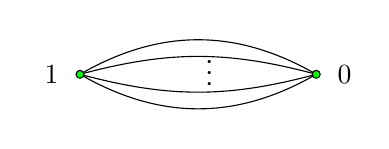
\begin{tikzpicture}[scale=.5]

\draw (0,0) to [out=330,in=210] (6,0) ;
\draw (0,0) to [out=345,in=195] (6,0) ;
\draw (0,0) to [out=15,in=165] (6,0) ;
\draw (0,0) to [out=30,in=150] (6,0) ;

\node [right] at (2.95,.25) {$\vdots$} ;

\draw [fill=green] (6,0) circle [radius=0.1cm] ;
\node [right] at (6.1,0) {$\;0$} ;
\draw [fill=green] (0,0) circle [radius=0.1cm] ;
\node [left] at (-.3,0) {$\;1$} ;

\end{tikzpicture}
\end{center}

For every $p$ and $r$, $\Jac(B_{p^r})\simeq\Z/p^r\Z$, and the pairing on $\Jac(B_{p^r})$ is isomorphic to the residue pairing.

\vspace{0.1in}
{\textcolor{purple}{\large{\bf{The nonresidue pairing}}}} \vspace{0.05in}\\
A candidate for getting the nonresidue pairing is the \textbf{cycle graph} $C_{p^r}$. Indeed $\Jac(C_{p^r})=\Z/p^r\Z$, and the pairing is isomorphic to $\pair{x}{y}=(-1)xy/p^r$.

However, it is not true that $-1$ is always a nonresidue modulo $p^r$. This is only true when $p\equiv 3\pmod 4$, so we must consider another construction when $p\equiv 1\pmod 4$. For this, the following claim is sufficient. 

\begin{claim*}
There exists $q$, a nonresidue mod $p$, such that $q^2<p^r$ and $q\equiv 3\pmod 4$ if $r$ is odd and $q\equiv 1\pmod 4$ if $r$ is even.
\end{claim*}
Given this claim, we pick $m$ such that $p^r\equiv m(q-m)\pmod q$, and construct the following \textbf{subdivided banana graph}:


%nr pairing for p=3mod4
\begin{center}
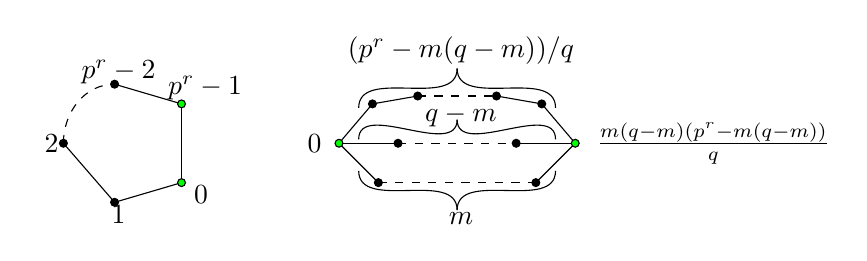
\begin{tikzpicture}[scale=.5]


\draw [dashed] (0,0) to [out=90,in=180] (1.3,1.5) ;
\draw (0,0) to (1.3,-1.5) ;
\draw (1.3,-1.5) to (3., -1) ;
\draw (1.3,1.5) to (3., 1) ;
\draw (3, -1) to (3, 1) ;

\draw [fill=green] (3,1) circle [radius=.1cm] ;
\node at (3.5, 1.4) {$\;p^r-1$} ;
\draw [fill=green] (3,-1) circle [radius=.1cm] ;
\node at (3.4, -1.3) {$\;0$} ;
\draw [fill] (1.3,1.5) circle [radius=.1cm] ;
\node at (1.3, 1.8) {$\;p^r-2$} ;
\draw [fill] (1.3,-1.5) circle [radius=.1cm] ;
\node at (1.3, -1.8) {$\;1$} ;
\draw [fill] (0,0) circle [radius=.1cm] ;
\node at (-.4,0) {$\;2$} ;

%subdivided banana
\draw [shift={(7cm,0cm)}] (0,0) to (1,-1) ;
\draw [shift={(7cm,0cm)}] (6,0) to (5,-1) ;
\draw [shift={(7cm,0cm)}] [dashed] (1,-1) to (5, -1) ;
\draw [shift={(7cm,0cm)}] (0,0) to (1.5,0) ;
\draw [shift={(7cm,0cm)}] (4.5,0) to (6,0) ;
\draw [shift={(7cm,0cm)}] [dashed] (1.5, 0) to (4.5, 0) ;
\draw [shift={(7cm,0cm)}] (0,0) to  (.85,1) ;
\draw [shift={(7cm,0cm)}] (.85,1) to (2,1.20) ;
\draw [shift={(7cm,0cm)}] (5.15,1) to (6,0) ;
\draw [shift={(7cm,0cm)}] (4,1.20) to (5.15,1) ;
\draw [shift={(7cm,0cm)}] [dashed] (2,1.2) to (4,1.2);
\draw [shift={(7cm,0cm)}] (.5, .1) to [out=90, in=-90] (3,.6) ; 
\draw [shift={(7cm,0cm)}] (5.5, .1) to [out=90, in=-90] (3,.6) ; 
\draw [shift={(7cm,0cm)}] (.5, -.7) to [out=-90, in=90] (3,-1.7) ; 
\draw [shift={(7cm,0cm)}] (5.5, -.7) to [out=-90, in=90] (3,-1.7) ; 
\draw [shift={(7cm,0cm)}] (.5, .9) to [out=90, in=-90] (3,1.9) ; 
\draw [shift={(7cm,0cm)}] (5.5, .9) to [out=90, in=-90] (3,1.9) ; 

\draw [shift={(7cm,0cm)}] [fill=green] (6,0) circle [radius=0.1cm] ;
\draw [shift={(7cm,0cm)}] [fill] (1.5,0) circle [radius=0.1cm] ;
\draw [shift={(7cm,0cm)}] [fill] (4.5,0) circle [radius=0.1cm] ;
\draw [shift={(7cm,0cm)}] [fill=green] (0,0) circle [radius=0.1cm] ;
\draw [shift={(7cm,0cm)}] [fill] (.85,1) circle [radius=0.1cm] ;
\draw [shift={(7cm,0cm)}] [fill] (2,1.2) circle [radius=0.1cm] ;
\draw [shift={(7cm,0cm)}] [fill] (4,1.2) circle [radius=0.1cm] ;
\draw [shift={(7cm,0cm)}] [fill] (5.15,1) circle [radius=0.1cm] ;
\draw [shift={(7cm,0cm)}] [fill] (1,-1) circle [radius=0.1cm] ;
\draw [shift={(7cm,0cm)}] [fill] (5,-1) circle [radius=0.1cm]  ;

\node [shift={(3.5cm,0cm)}] [left]  at (-.2,0) {$0$} ;
\node [shift={(3.5cm,0cm)}] [right] at (6.1,0) {$\;\frac{m(q-m)(p^r-m(q-m))}{q}$} ;
\node [shift={(3.5cm,0cm)}] at (3, .7) {$\;q-m$} ;
\node [shift={(3.5cm,0cm)}] at (3, -1.9) {$\;m$} ;
\node [shift={(3.5cm,0cm)}] at (3, 2.35) {$\;(p^r-m(q-m))/q$} ;

\end{tikzpicture}
\end{center}

This construction gives us the nonresidue pairing on $\Z/p^r\Z$ with $p\equiv 1\pmod 4$, provided that the above claim holds. For $r\ge2$, we have a proof of this claim. In the case that $r=1$, the \textbf{Generalized Riemann Hypothesis} implies the result. 


\end{multicols}

}

\end{poster}%
%
\end{document}
